\documentclass{article}
\usepackage{amsmath,amssymb}
\usepackage{mathtools}
\usepackage{amsfonts}
\usepackage{amssymb}
\usepackage{tikz}

\DeclarePairedDelimiter{\ceil}{\lceil}{\rceil}
\newcounter{question}
\setcounter{question}{0}
\begin{document}

\newcommand\Que[1]{%
   \leavevmode\par
   \stepcounter{question}
   \noindent
   \thequestion. Q --- #1\par}

\newcommand\Ans[2][]{%
    \leavevmode\par\noindent
   {\leftskip37pt
    A --- \textbf{#1}#2\par}}

\Que{
    Let $V$ be the set of all $0–1$ sequences of length d. 
    The graph on $V$ in which two such sequences form an edge 
    if and only if they differ in exactly one position is called the 
    \textit{d-dimensional cube}. 
    Determine the average degree, number of edges, and the length of
    a smallest cycle in this graph.
    }
\Ans{
    Let's visualize the graph $ G = (V,E) $ for \textit{dimension}, $d=3$.\\\\

    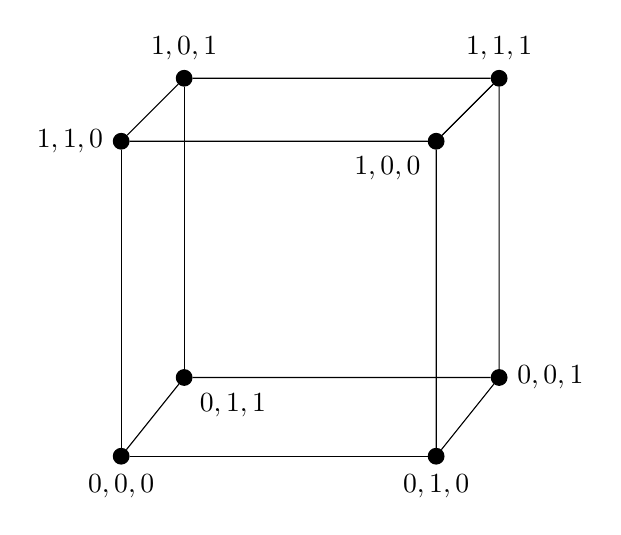
\begin{tikzpicture}
        \foreach \n/\x/\l/\p in{
        1/{( 0  , 0)}/{$0,0,0$}/below,
        2/{( 4, 0)}/{$0,1,0$}/below,
        3/{( .8, 1)}/{$0,1,1$}/south east,
        4/{( 4.8, 1)}/{$0,0,1$}/right,
        5/{( 0, 4)}/{$1,1,0$}/left,
        6/{( 4, 4)}/{$1,0,0$}/south west,
        7/{( 0.8, 4.8)}/{$1,0,1$}/above,
        8/{( 4.8, 4.8)}/{$1,1,1$}/above
        }
        {
            \node[inner sep=2pt,
            circle,draw,fill,label={\p:\l}] 
            (\n) at \x {};
        }
        \draw (1) -- (2) -- (6) -- (5) -- (1);
        \draw (5) -- (6) -- (8) -- (7) -- (5);
        \draw (2) -- (4) -- (8) -- (6) -- (2);
        \draw (1) -- (3) -- (4);
        \draw (3) -- (7);
    \end{tikzpicture}\\

    \underline{\textbf{Features (for $3$ dimensions):}}\\

    \textbf{Dimensions}, $d=3$\\

    \textbf{Number of vertices}, $ [V] = 2^{d} = 8 $\\

    \textbf{Number of edges}, $ [E] = 12 (=\frac{8\times{3}}{2}) $\\

    \textbf{Length of smallest cycle}, $ = 4 $\\
    
    \textbf{Average degree}, $ deg_{G}(v) = 3 $\\\\


    \underline{\textbf{features (For $d$ dimensions):}}\\

    \textbf{Number of vertices}, $ [V] = 2^{d} $\\

    \textbf{Number of edges}, $ [E] = \frac{[V]\times{d}}{2} $
    [$\because$ for a sequence of length $d$, 
    there are exactly $d$ ways to change exactly $1$ bit 
    ($0$ or $1$) and derive $d$ neigbors for each vertex.
    We divide the result by $2$ because each vertex 
    would be counted twice.]\\

    \textbf{Length of smallest cycle}, $ = d+1 $\\

    \textbf{Average degree}, $ deg_{G}(v) = d $, 
    since every vertex is connected to exactly $d$ 
    other vertices.\\
    }
\end{document}